% !TeX spellcheck = en_GB
% =================================================================
\chapter{Analysis of Available Data Sources and Techniques}
\label{chap:analysis}

\todo[defer,inline]{introduce this chapter}

\dots

Before we start, we need to define the central term \emph{metadata}.
For this purpose, we follow \citeauthor{Hider2008}'s \autocite*{Hider2008} definition and reflection:
The term \emph{metadata} is used in multiple ways.
The most general use is according to its literal meaning, \enquote{data about data}.
This definition is not restricted to the library domain
but includes bibliographic records for documents (which contain the primary \emph{data}).
A more specific variant is the use of \enquote{metadata} to refer to
structured data describing digital objects,
again independently of the library domain. \citeauthor{Hider2008} also note that
these two meanings can no longer be clearly distinguished in view of the
progressing digital transformation. In this thesis, we adopt their
decision to use the term \emph{metadata} in the most general sense,
\enquote{applying to all information resources} \autocite[p.13]{Hider2008}.


% -----------------------------------------------------------------
\section{Data Formats and Communication Protocols}
\label{sec:data_models}


In this section, we describe standards, data models, and formats that are used in the data sources
relevant for our work. 

% - - - - - - - - - - - - - - - - - - - - - - - - - - - - - - - - -
\subsection{Standards for the Description of Bibliographic Resources}

% .............
\paragraph{FRBR.}

The \gls{FRBR} constitute a conceptual entity-relationship model
developed by the \gls{IFLA} in 1998 (and updated in 2009)
in order to support users in finding, identifying, selecting, and accessing
bibliographic items \autocite[p.17]{Wiesenmueller2015}.
\gls{FRBR}'s entities represent things that need to be represented in the data.
These entities fall into three groups, of which we discuss the first
two.
Entities of Group~1 are \term{Work}, \term{Expression}, \term{Manifestation}, \term{Item},
and their common superordinate concept \term{Endeavour};
entities of Group~2 are \term{Person}, \term{Family}, \term{Corporate body},
and their superordinate concept \term{Responsible\_entity}.
Furthermore, \gls{FRBR} contains relations that link Group-1 entities with each other
and with Group-2 entities, respectively.
All these entities and relations are shown in Figure~\ref{fig:FRBR}.

\begin{figure}[ht]
  \centering
  
\includegraphics[height=60mm]{img/FRBR_Group1.png}
  \qquad
  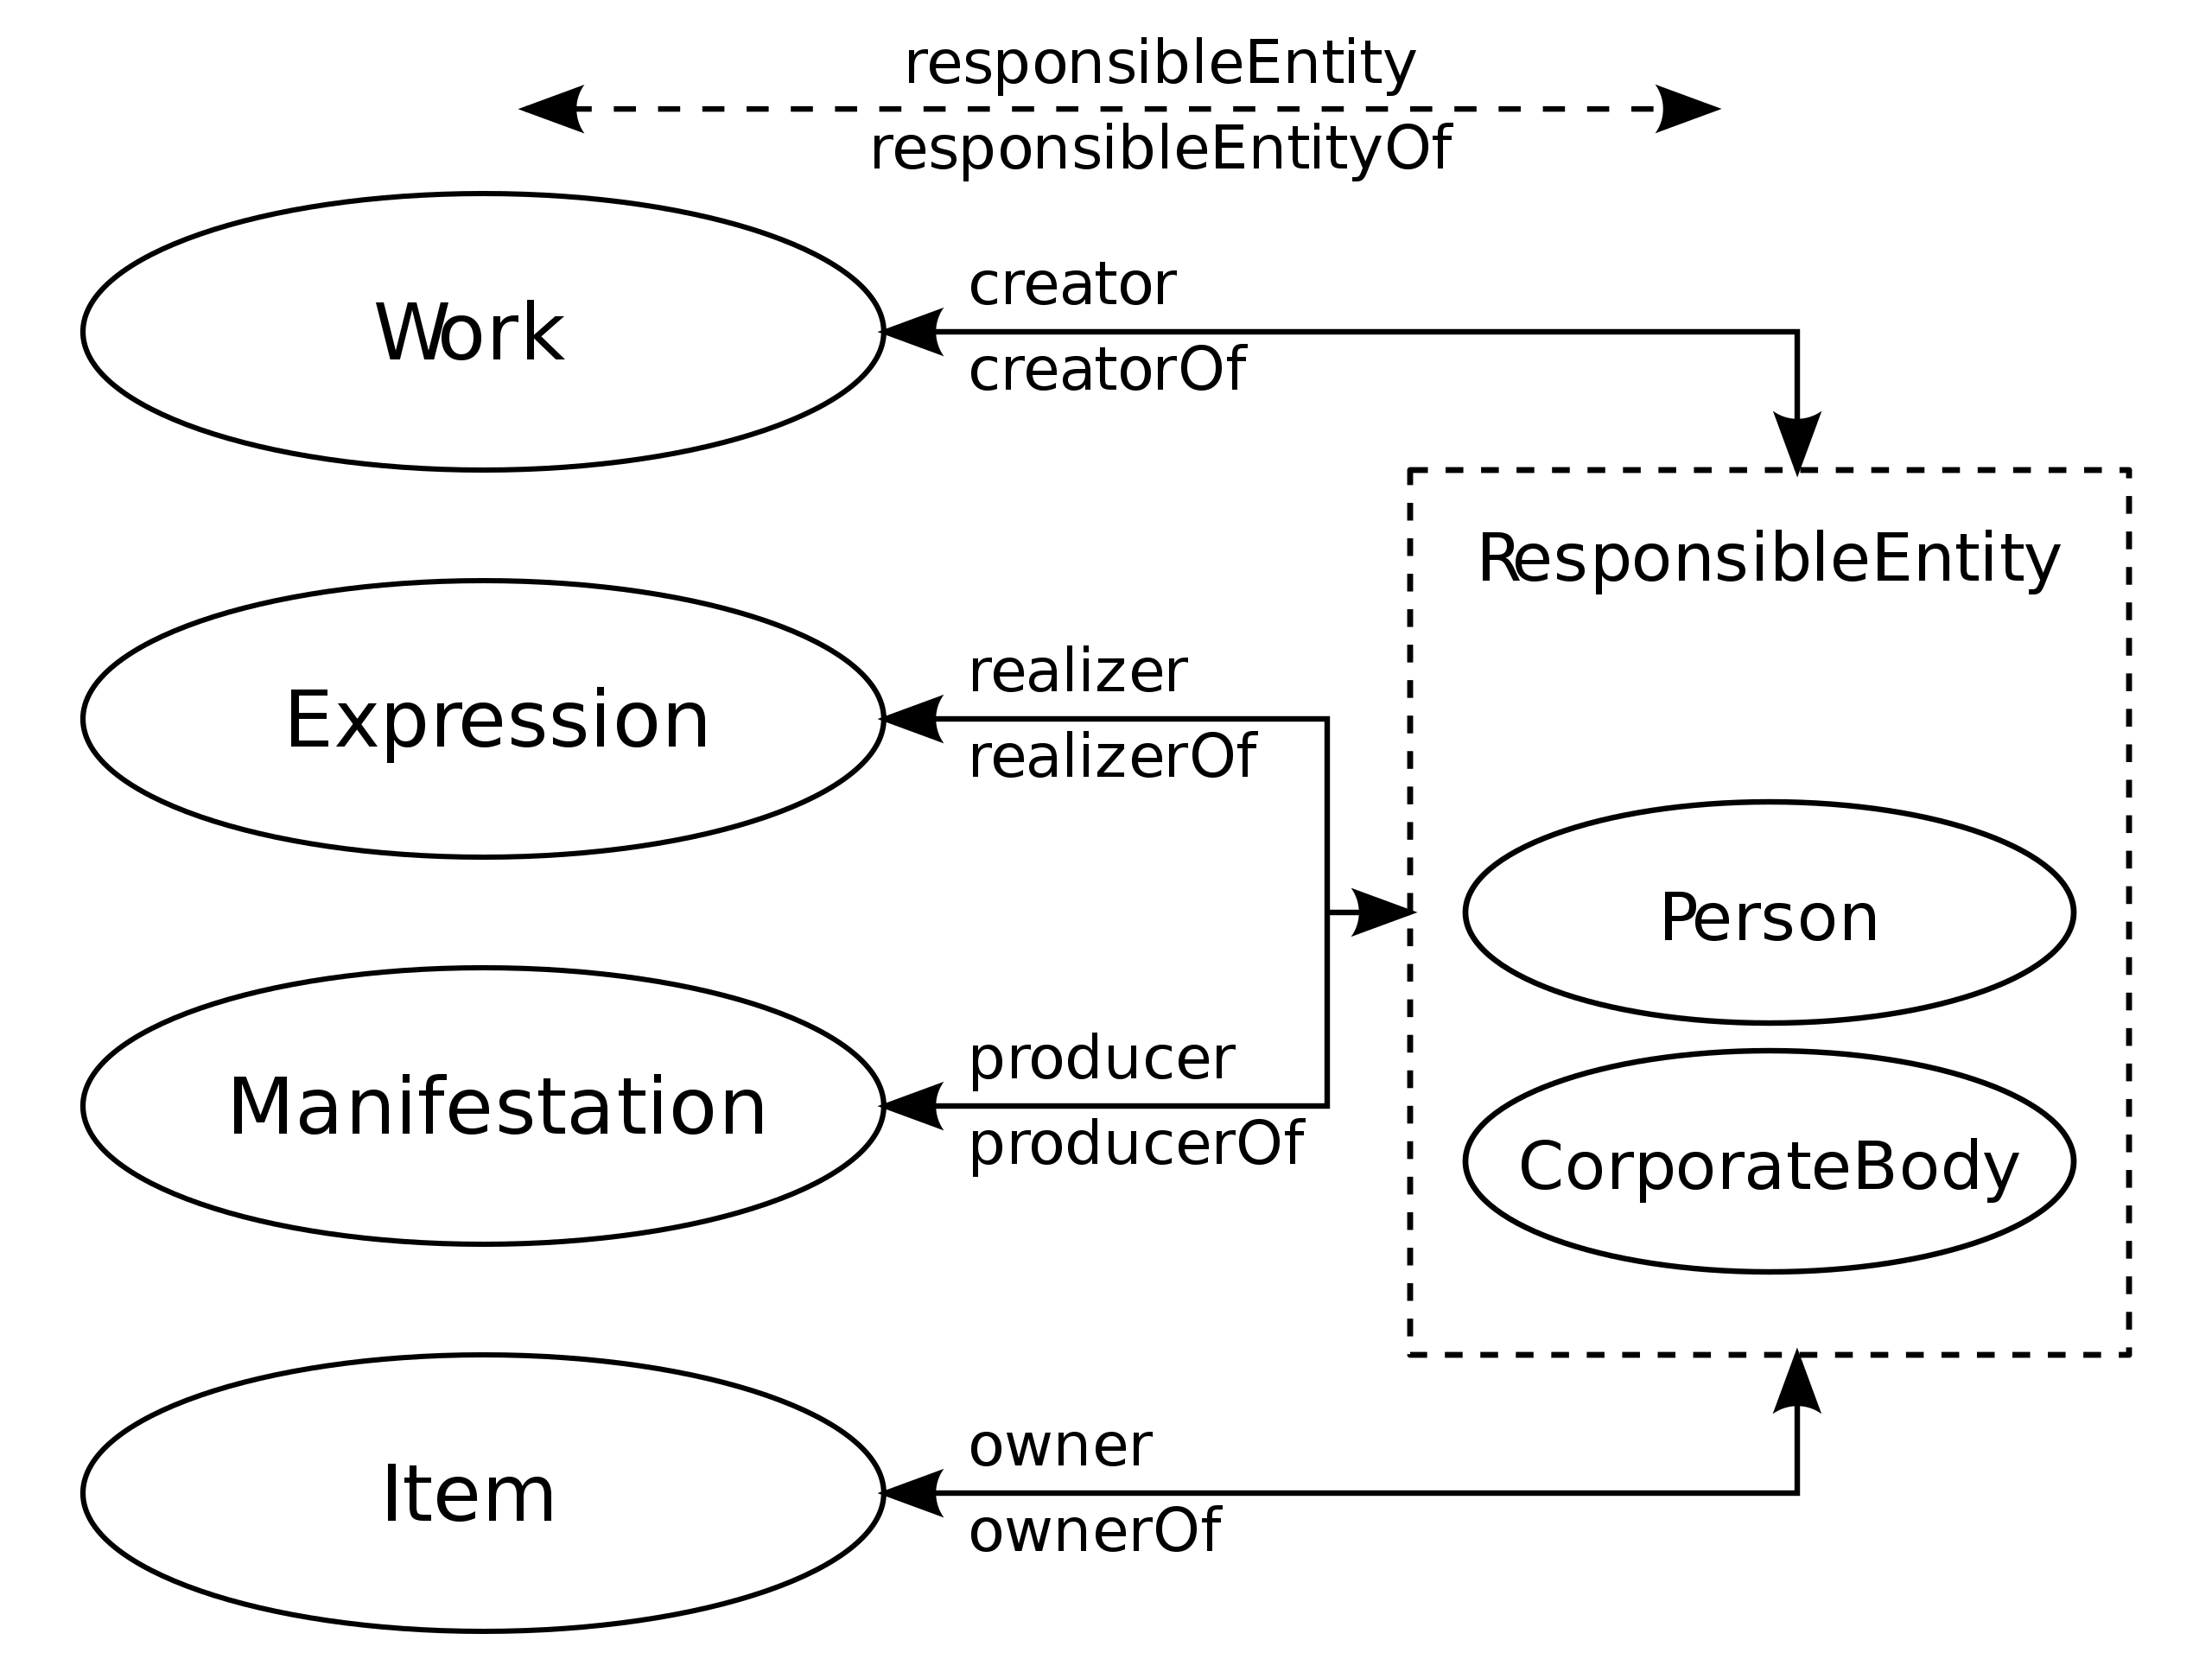
\includegraphics[height=60mm]{img/FRBR_Group2.png}
  
  \caption[Basic FRBR entities and relations of Group~1 and Group~2]{%
    \parbox[t]{.85\linewidth}{%
      Basic \gls{FRBR} entities and relations of Group~1 (left) and Group~2 (right)
      \par
      \begin{footnotesize}
        \href{https://commons.wikimedia.org/wiki/File:FRBR-Group-1-entities-and-basic-relations.svg}{\enquote{Basic Group 1 entities and relations of the FRBR model (RDF version)}} and
        \href{https://commons.wikimedia.org/wiki/File:FRBR-Group-2-entities-and-relations.svg}{\enquote{Basic Group 2 entities and relations of the FRBR model (RDF version)}}
        by \href{https://commons.wikimedia.org/wiki/User:JakobVoss}{Jakob Voss} are licenced under \href{https://creativecommons.org/licenses/by-sa/4.0/}{CC BY-SA 4.0}.
        \par
      \end{footnotesize}
    }%
  }
  \label{fig:FRBR}
\end{figure}

The \gls{IFLA} also developed
a conceptual entity-relationship model for authority data,
the \gls{FRAD},
as well as a continuation of FRBR,
the \gls{FRSAD}.

FRBR serves as a basic principle of RDA, which we discuss next.

% .............
\paragraph{RDA.}

\gls{RDA} is a standard for the cataloguing of publications
in cultural heritage institutions, and particularly in libraries.
RDA is implemented and used in the library systems of several countries, including
the US, the UK, Canada, Australia, and the German-speaking countries
\autocite{WikiDE_RDA}.

RDA and the application guidelines for the German-speaking area
stipulate a special practice for recording FRBR Group-1 entities and relating 
them to each other: Bibliographic records (\enquote{Titeldatensätze})
have a bibliographic level for describing a manifestation
and an exemplar level for describing the related exemplars. The description of works and expressions
is considered part of the description of a manifestation and thus recorded on the bibliographic level.
However, it is possible to create and link an authority record for a work or expression
containing the relevant description. In that case, the source of the information can be recorded as well
\autocite[cf.][§5.1]{Wiesenmueller2015}.

For our approach, this observation means that catalogues of German libraries
do not use a uniform way of linking, e.g., a work $X$ with its manifestations.
In particular, if there is no authority record for $X$,
then $X$ is represented in the data of its manifestations only implicitly 
(and possibly ambiguously).

% - - - - - - - - - - - - - - - - - - - - - - - - - - - - - - - - -
\subsection{Data Communication Protocols}

% .............
\paragraph{Z39.50}

\dots

% .............
\paragraph{SRU}

\dots

\url{https://en.wikipedia.org/wiki/Search/Retrieve_via_URL}, \url{https://www.loc.gov/standards/sru/}

% .............
\paragraph{OAI-PMH}

\dots

% - - - - - - - - - - - - - - - - - - - - - - - - - - - - - - - - -
\subsection{Data Description Schemata}

% .............
\paragraph{MARC}

\dots

(21, XML, Turbomarc, MAB2 as a MARC \enquote{family member} \autocite[p.204]{Hider2008})

% .............
\paragraph{DC.}

\gls{DC} is an international standard consisting of 15 essential metadata terms
for describing digital or physical resources.
It was formulated by the \gls{DCMI}, a project of the US-American non-profit organisation
ASIS\&T, for the purpose of locating information resources on the Web.\todo[quick]{\enquote{(World Wide) Web} $\to$ \enquote{WWW} (globally)}
The 15 core elements are tailored towards the \enquote{primary metadata needs} across domains
\autocite[p.215]{Hider2008}, thus making it a flexible data model.
Applications of \gls{DC} include resource description,
the combination of metadata vocabularies from different standards,
and the provision of interoperability in the linked data context.
\gls{DC} is extended by the \emph{DCMI Metadata Terms}.
Sources of this summary are \textcite[§§1, 10]{Hider2008},
and \citeauthor{WikiDC}~\autocite{WikiDC}.

\todo[inline]{DC vs. MARC, \autocite[§10]{Hider2008}?}

% .............
\paragraph{MODS}

\dots

% .............
\paragraph{RDF}

\dots

\todo[inline]{if necessary, discuss PICA, BIBFRAME \url{https://en.wikipedia.org/wiki/BIBFRAME}}


% -----------------------------------------------------------------
\section{Data Sources}
\label{sec:data_sources}

We have searched the literature and the Web for data sources that contain information
relevant for provenance research, i.e., works, expressions, manifestations, exemplars,
persons, ownership, social relationships, and more. 
We decided to put a slight focus on data sources from the German-speaking area, 
aiming at a selection of data sources that is manageable in the context of a master's thesis,
and influenced by the selection in the \gls{SoNAR} project (see Section~\ref{sec:HNA+SoNAR}).
In the following, we will first give an overview of these data sources
and then provide more information about some of them,
including their scope and the technical infrastructure provided.
This list is not exhaustive and needs to be extended
as soon as our model is implemented in a concrete tool in future work.

% - - - - - - - - - - - - - - - - - - - - - - - -
\subsection{Collection of Data Sources}

We have identified four categories of relevant data sources:
library catalogues, special databases for provenance research, authority files, and knowledge bases.
We next describe, for each of these categories, the relevant information that is
contained in the respective data sources, and we list examples.

% .............
\paragraph{Library Catalogues}
%
%Library catalogues 
contain the following information relevant for provenance research.
%
\begin{itemize}
  \item
    bibliographic entities (works, manifestations, expressions, exemplars)
  \item
    relations between these entities (e.g., \term{isManifestationOf})
  \item
    attributes for these entities (e.g., year of publication)
  \item
    people and corporate bodies and relations such as authorship
  \item
    provenance entries (including, e.g., owners, the ownership relation, and further attributes such as the year of ownership)
  \item
    (implicitly) the current ownership
  \item
    (ideally) references to entries in authority files for all these types of entities
\end{itemize}
%
Examples of relevant library catalogues include:
%
\begin{itemize}
  \item
    catalogues of national libraries, which often aim at collecting literature exhaustively
    and which are most likely to make metadata available in interoperable formats;
    in particular: \gls{DNB}, \gls{LoC}, British Library
  \item
    meta-catalogues that enable a federated search in several catalogues;
    in particular: WorldCat and \gls{KVK}
  \item
    catalogues of (German) library networks;
    in particular: \gls{K10plus}, 
    \glsunset{B3KAT}\gls{B3KAT},
    \glsunset{hbz}%
    \glsunset{hebis}%
    and the union catalogues of \gls{hbz} and \gls{hebis}
  \item
    catalogues of single libraries, if not covered by any of the above
  \item
    special catalogues;
    in particular: \gls{ZDB}, \gls{KPE}, \gls{ZEFYS}, ExilePress (which have been used in the \gls{SoNAR} project) \todo{explain; relate to SoNAR or loot research}
\end{itemize}

% .............
\paragraph{Authority Files}
%
%Authority files
contain the following information relevant for provenance research.
%
\begin{itemize}
  \item
    entities such as persons, corporate bodies, places, works
  \item
    relations such as social relations, family relations, professional relations
  \item
    attributes for the entities such as their profession
\end{itemize}
%
They are usually subject to a strict quality control.
Examples include the \gls{GND} in the German-speaking area (which has been used extensively in \gls{SoNAR}),
the \gls{LCNAF} for North America,
and \gls{ISNI} and \gls{VIAF} worldwide.

% .............
\paragraph{Knowledge Bases.}

According to the insights from the \gls{SoNAR} project,
(open) \glspl{KB} can be useful when trying to overcome the problem with missing or unbalanced data
in authority files such as the \gls{GND} (see Section~\ref{sec:HNA+SoNAR}).
\Glspl{KB} are usually edited independently of the library domain by a wider community of contributors,
and their quality cannot be expected to meet the standards of catalogues or authority files edited by library personnel.
A prominent example of an open, cross-domain \gls{KB} is Wikidata,
which has tentatively been used in the context of the \gls{SoNAR} project.

% .............
\paragraph{Cultural Heritage Databases.}

This category contains generic federated portals of cultural heritage items
as well as special databases created especially for the support of provenance research.
Examples for these two kinds of databases are, respectively, Europeana (see Section~\ref{sec:linked_data+integration})
and Proveana---the research database of the German Lost Art Foundation \autocite{Proveana}.

% - - - - - - - - - - - - - - - - - - - - - - - -
\subsection{Analysis of Data Sources}

We now provide a review of the following data sources from the previous list:
\gls{DNB}, \gls{KVK}, \gls{K10plus}, \gls{ZDB}, \gls{KPE}, \gls{GND}, Wikidata, Proveana, and Europeana.
The main goal of this analysis is to provide an exemplary overview of the features and specifics
of these data sources, and to inform the model that we will develop in the subsequent chapter.
In order to fulfil this purpose, it is not necessary to review all data sources listed above
exhaustively.

We collect the following information for each data source.
%
\begin{itemize}
  \item
    \emph{Scope:}~
    thematic focus; coverage; number of records; standards for cataloguing
  \item
    \emph{Technical infrastructure:}~
    data format; data model; interfaces; support for linked data
  \item
    \emph{Data quality (from the \gls{SoNAR} grant proposal \autocite[p.\,19ff.]{SchneiderKempf2018}),
    if applicable:}~
    use of persistent identifiers and URIs; adherence to standards for, e.g., time and date specification
  \item
    \emph{features useful in the context of \gls{SoNAR} (see our discussion in Section~\ref{sec:insights_from_SoNAR}), if applicable:}~
    recording of temporal attributes or relations; recording of data provenance
  \item
    further features specific to the respective data source, if applicable
\end{itemize}

% .............
\paragraph{DNB.}

The following information is taken from the \gls{DNB}'s websites under the category \enquote{DNB Professional} \autocite{DNB_coll_mand,DNB_cataloguing,DNB_metadata}.

The DNB adheres to a legal collection mandate, according to which
the DNB collects \enquote{all texts, images and sound recordings published in Germany or in the German language, translated from German or relating to Germany that have been issued since 1913}  \autocite{DNB_coll_mand}. This includes all physical publications, and, since 2006, electronic publications made available via the internet. The mandate commits the DNB to a complete and unbiased collection that includes, among others, \enquote{printed works compiled or published between 1933 and 1945 by German-speaking emigrants} \autocite{DNB_coll_mand}.

The DNB catalogues its entire collection both descriptively and by subject, 
adhering to standards such as \gls{RDA}, using authority data, and including persistent identifiers such as ISBN, ISSN, URN, and DOI.
The cataloguing data feeds the German National Bibliography.

According to the 2021 annual report \autocite{DNB_Jahresbericht_2021},
the DNB's holdings comprise 43.7 million physical or digitally accessible units, 
which are represented by almost 26 million records in the German National Bibliography.

Metadata can be obtained from the DNB freely (under the CC0 1.0 licence) via the interfaces
\gls{SRU} and \gls{OAI}, which support XML serialisations of the data formats
MARC~21, \gls{RDF}, DNB Casual (an XML-based \gls{DC} format), and MODS.\todo{introduce all these abbreviations}
Further data formats are available via an individual access
to the \enquote{Data Shop}.
The DNB's Linked Data Service provides open access to its bibliographic and authority data
in RDF under the Creative Commons Zero (CC0 1.0) license. Instructions on how to use these interfaces
are given on the DNB's webpage on metadata services \autocite{DNB_metadata}.

According to the detailed specifications on the MARC format by the DNB
\autocite{DNB_MARC21,DNB_MARCXML}, the recording of dates and times, languages,
geographic area codes, and countries conforms to ISO standards (8601, 639-1, 3166).
Since 2015, the DNB has been using MARC field 883
for recording the metadata provenance for a selection of data fields
\autocite{DNBwiki_MARC_883}.

\todo[inline]{more comments on consequences of using RDA (works/expressions)?}

\todo[inline]{temporal data restricted to year of publication?}

% .............
\paragraph{WorldCat}

\dots

% .............
\paragraph{KVK}

\dots

% .............
\paragraph{K10plus}

is the joint catalogue of the German library networks GBV and SWB.
Together, these two networks comprise more than 1400 national, regional,
academic, and public libraries \autocite{BSZGBV,GBV_VZG},
of which 838 participate in \gls{K10plus}, according to the list of participating institutions
in the K10plus Wiki \autocite{K10plusWiki}. Thus, \gls{K10plus} comprises the data from
the majority of German academic institutions \autocite[cf.][]{BSZ_K10plus}.

Cataloguing in K10plus adheres to the same standards as in the DNB.
As of 31 December 2022, K10plus contains 80.8 million bibliographic records (\enquote{Titeldatensätze})
with 235.4 million ownership records \autocite{GBV_K10plus_Statistik}.

K10plus provides metadata freely (under the CC0 1.0 licence),
mainly via the interfaces Z39.50 and SRU.
Those support the data formats MARC~21, MARC-XML (and its variant Turbomarc),
PICA+, PICA-XML, \gls{DC}, and MODS (and the legacy format MAB2).
Detailed instructions on how to use these interfaces
are given in the K10plus Wiki \autocite{K10plusWiki}.
In addition, snapshots of K10plus data are provided regularly
in MARC-XML and as linked open data (RDF-XML), but the information
on these in the K10plus Wiki is incomplete \autocite{K10plusWikiOD}.



\dots

\todo[inline]{discuss provenance indexing}

\todo[inline]{GND data accessible via the same interface? Prepare for GND section below}


% .............
\paragraph{ZDB}

\dots

% .............
\paragraph{KPE}

\dots

% .............
\paragraph{GND.}

The \gls{GND} is operated by the \gls{DNB}
\enquote{in cooperation with many other libraries, libra[r]y networks and other cultural and academic institutions.
At present, the GND contains around 9 million authority records for persons, corporate bodies, congresses, geographic entities, specialised terms and works; these are supplemented, updated and used frequently} \autocite{DNB_cataloguing}. More detailed statistics can be found in the DNB's
2021 annual report \autocite[p.49]{DNB_Jahresbericht_2021}.
GND adheres to the same cataloguing standards and offers the same technical infrastructure
as the DNB catalogue; in particular, GND data is accessible alongside DNB data
via the same interfaces and data formats, including RDF.

\todo[inline]{temporal data restricted to year of publication or years of birth and death, if available? No temporal attributes on relations (e.g., student, coauthor) $\Longrightarrow$ first review K10plus guidelines for cataloguing authority data!}


\todo[inline]{add insights from SoNAR (§~\ref{sec:HNA+SoNAR}) and DHa (see below)}

DHa's remarks on GND vocabulary and richness of GND data:
%
\begin{itemize}
  \item
    \emph{Individualisierungsregeln}: relationships to other people are given in order to uniquely
    identify the current person; there is no obligation to record relationships
    (and GND does not claim to be an encyclopedia)
  \item
    relations are not normed:
    e.g., field \enquote{Funktionsbezeichnung}: \$4 code \enquote{Eigenschaft der Beziehung},
    specified by \$v \enquote{Freitext}
  \item
    professions are recorded in 678 \$b \enquote{biographische Anmerkung(en)} --
    historically in free text,
    more recently via link to the GND authority data for the respective profession (i.e., more standardised)
  \item
    Tp1 datasets: field 65 (6J?) \enquote{GND Systematik: eingeschr. Tätigkeit} (?),
    query level 1 datasets?
  \item
    $\leadsto$ \mybold{look/read all this up!}
\end{itemize}


\dots


% .............
\paragraph{Wikidata}

\dots

% .............
\paragraph{Proveana}

\dots

% .............
\paragraph{Europeana}

\dots

\par\bigskip
\todo[inline]{Take the following points into account ::}

\begin{itemize}
  \item
    \mybold{KVK} (\enquote{federated search}: shallower than in single catalogues,
    but (sufficient) information on all copies!);
    further catalogues?
  \item
    more from \gls{SoNAR} , see report on WP 2 (in particular details on p.23f.).
    Get back to the discussion on \gls{GND} and further data sources in Section~\ref{sec:HNA+SoNAR}.
  \item
    see also the list by \autocite{Menzel2020}:

    \blockquote{%
      \begin{itemize}
        \item
          The Integrated Authority File (GND) represents and describes 8,295,047 entities (people, corporations, conferences, geographical areas, technical terms, and works);
        \item
          The German National Library (DNB) provides descriptions of bibliographic resources. The dataset has 19,926,573 records of books, magazines, newspapers, sheet music, music recordings, audio books etc.;
        \item
          The German Union Catalogue of Serials (ZDB) describes newspapers, magazines, serial titles, yearbooks, etc. and contains 1,908,334 records;
        \item
          The Kalliope Union Catalog (KPE) is a collection of personal papers, manuscripts, and publishers’ archives, which consists of 26,752 records;
        \item
          The Newspaper Information System (ZeFYS) represents 2,596,641 digitized pages of historical newspapers and full texts;
        \item
          The Exile Press represents German-language exile journals between 1933 and 1945 and consists of 5,336 digitized pages.
      \end{itemize}
    }
  \item
    further criteria: arity of relationships, data formats, temporal data?
  \item
    also clarify: does the structure of these data sources support the model to be developed?
  \item
    focus the following considerations on a narrow choice of these data sources;
    the general approach to be developed should be largely independent on that concrete choice
  \item 
    in-depth analysis of data sources (e.g., overlap and differences) is worthwhile
    but must be deferred to future work
\end{itemize}

% -----------------------------------------------------------------
\section{Data Integration and Further Techniques}
\label{sec:data_integration}

\begin{itemize}
  \item 
    ETL (from grant proposal \gls{SoNAR}, p.~8, AP1-1)
  \item
    upper-level ontologies?
  \item 
    ontologies on research
  \item
    FRBRoo?
  \item
    \gls{RDF}, SPARQL, N-Quads?
\end{itemize}


\dots

% -----------------------------------------------------------------
\section{Implications on Modelling}
\label{sec:implications_on_modelling}

\dots


\begin{itemize}
  \item
    \mybold{constants plus unary and binary relationships suffice (?) -- evidence: FRBR, DC(?), works on graph techniques in HNA, data sources (e.g., DNB, GND (linked data services?), K10plus?)}
  \item 
    uniform vs.\ distributed scenario?
    %
    \begin{itemize}
      \item
        distributed: data source graph is implicit; data sources are queried \enquote{on the fly}
        (this is the preferred scenario here; see delineation from SoNAR in §\ref{sec:HNA+SoNAR})
      \item
        uniform: data source graph is generated explicitly (using data integration techniques)
        and updated in fixed intervals
    \end{itemize}
    %
\end{itemize}


